\documentclass[UTF8,zihao=-4,fontset=none,scheme=chinese,openany,twoside]{ctexbook}
% ===================================================================
%  《月之都——〈广寒宫残简〉辑佚与考释》专用版式
%
%  丛书基座在 ../../shared/style/series-base.tex；本书只在这里追加
%  本书特有的东西。跨书共用的东西一律改基座，不要改这里。
% ===================================================================

% ===================================================================
%  远东异端史料与文明起源重构丛书 · 版式基座（series-base）
%
%  兄弟书目共用此文件。改这里 = 改全套书。
%  各书在自己的 preamble.tex 里 \input 本文件，再追加本书特有的定义。
%
%  体例：仿苏式/中译社科类古籍。16 开 185×260 mm，版心 147×214 mm。
%  依赖：XeLaTeX + ctex + xeCJK + zhnumber + Noto Serif/Sans CJK SC
% ===================================================================

\usepackage{geometry}
\geometry{
  paperwidth=185mm, paperheight=260mm,
  inner=21mm, outer=17mm, top=22mm, bottom=24mm,
  headheight=24pt, headsep=6.5mm, footskip=11mm
}

\usepackage{fontspec}
\usepackage{xeCJK}
\usepackage{xcolor}
\usepackage{graphicx}
\usepackage{array,tabularx,booktabs,multirow,makecell}
\usepackage{longtable}
\usepackage{multicol}
\usepackage{calc}
\usepackage{amsmath,amssymb}
\usepackage{enumitem}
\usepackage{fancyhdr}
\usepackage{titlesec}
\usepackage{titletoc}
\usepackage{tcolorbox}
\tcbuselibrary{skins,breakable}
\usepackage[perpage]{footmisc}
\usepackage{etoolbox}
\usepackage{eso-pic}
\usepackage{tikz}
\usetikzlibrary{patterns,arrows.meta,calc,positioning,decorations.pathmorphing,
                decorations.markings,shapes.geometric}
\usepackage{pgfplots}
\pgfplotsset{compat=1.17}
\usepackage{caption}
\usepackage[hidelinks,bookmarksnumbered,bookmarksopen]{hyperref}

% ---------------------------------------------------------------- 颜色
\definecolor{ink}{HTML}{17191C}
\definecolor{graphite}{HTML}{3F454C}
\definecolor{pencil}{HTML}{5B6167}
\definecolor{rulegrey}{HTML}{8B8F93}
\definecolor{faintgrey}{HTML}{C9C9C4}
\definecolor{oxblood}{HTML}{6E1B22}
\definecolor{coverbg}{HTML}{1A1C20}
\definecolor{coverink}{HTML}{E6DFCF}
\definecolor{coverdim}{HTML}{7C7A73}
\definecolor{shade}{HTML}{F2F0EA}
\definecolor{stamp}{HTML}{8C2B2B}

\color{ink}

% ---------------------------------------------------------------- 字体
\setmainfont{NotoSerif}[
  Extension=.ttf,
  UprightFont=*-Regular,
  BoldFont=*-Bold,
  ItalicFont=*-Italic,
  BoldItalicFont=*-BoldItalic,
  Path=/usr/share/fonts/noto/
]
\setsansfont{NotoSans}[
  Extension=.ttf,
  UprightFont=*-Regular,
  BoldFont=*-Bold,
  ItalicFont=*-Italic,
  BoldItalicFont=*-BoldItalic,
  Path=/usr/share/fonts/noto/
]
\setmonofont{JetBrains Maple Mono}[
  UprightFont=* Regular, BoldFont=* Bold, Scale=0.92
]

\setCJKmainfont{Noto Serif CJK SC}[
  BoldFont=Noto Serif CJK SC Bold,
  ItalicFont=Noto Serif CJK SC,
  BoldItalicFont=Noto Serif CJK SC Bold
]
% 让罗马数字、带圈数字等“类汉字”符号使用中文字体
\xeCJKDeclareCharClass{CJK}{"2150 -> "218F, "2460 -> "24FF, "3000 -> "303F}

% 标点用开明式：行首禁则与压缩都较默认的 plain 更稳，可减少「句号独行」。
\AtBeginDocument{\xeCJKsetup{PunctStyle=kaiming}}

\setCJKsansfont{Noto Sans CJK SC}[BoldFont=Noto Sans CJK SC Bold]
\setCJKmonofont{Noto Sans Mono CJK SC}

% 伪斜体的字距（中文无真斜体，此处仅作强调标记）
\newcommand{\jia}{\CJKfontspec{Noto Serif CJK SC}}

% ---------------------------------------------------------------- 版心
\linespread{1.42}
\setlength{\parindent}{2em}
\setlength{\parskip}{0pt}
\raggedbottom
\setlength{\emergencystretch}{2em}
\clubpenalty=10000
\widowpenalty=10000

% ---------------------------------------------------------------- 计数
\renewcommand{\thechapter}{\chinese{chapter}}
\renewcommand{\thesection}{\chinese{section}}
\renewcommand{\thesubsection}{\chinese{subsection}}
\renewcommand{\thefigure}{\arabic{chapter}-\arabic{figure}}
\renewcommand{\thetable}{\arabic{chapter}-\arabic{table}}
\renewcommand{\theequation}{\arabic{chapter}-\arabic{equation}}

% ---------------------------------------------------------------- 章标题
\newcommand{\chapterornament}{%
  \vspace{0.8\baselineskip}%
  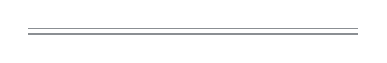
\begin{tikzpicture}[baseline=0pt]
    \fill[rulegrey] (0,0) rectangle (42mm,0.75pt);
    \fill[rulegrey] (0,2.4pt) rectangle (42mm,2.75pt);
  \end{tikzpicture}}

\titleformat{\chapter}[display]
  {\centering\normalfont}
  {\large\mdseries 第\,\thechapter\,章}
  {0.55\baselineskip}
  {\normalfont\LARGE\bfseries\linespread{1.15}\selectfont}
  [\chapterornament]
\titlespacing*{\chapter}{0pt}{-16pt}{30pt}

\titleformat{\section}
  {\normalfont\sffamily\large\bfseries\linespread{1.2}\selectfont}
  {第\,\thesection\,节}{0.6em}{}
\titlespacing*{\section}{0pt}{18pt}{9pt}

\titleformat{\subsection}
  {\normalfont\normalsize\bfseries}
  {\thesubsection、}{0.2em}{}
\titlespacing*{\subsection}{0pt}{13pt}{6pt}

\titleformat{\subsubsection}
  {\normalfont\normalsize\itshape}
  {}{0pt}{}
\titlespacing*{\subsubsection}{0pt}{10pt}{4pt}

% 章题下的俄文原题
\newcommand{\chaptersubtitle}[2]{%
  \begin{center}
  \vspace{-14pt}
  {\small\sffamily\color{pencil}#1}\\[2pt]
  {\small\sffamily\itshape\color{pencil}#2}
  \end{center}
  \vspace{4pt}
}

% 章前题记
\newcommand{\epigraphbox}[2]{%
  \begingroup
  \vspace{2pt}
  \begin{list}{}{\leftmargin=3.2em \rightmargin=2.2em \topsep=0pt
                 \parsep=0pt \itemsep=0pt}
  \item\relax
  {\small\linespread{1.32}\selectfont\color{ink!88}#1\par}
  \vspace{3pt}
  {\small\raggedleft\color{pencil}#2\par}
  \end{list}
  \vspace{6pt}
  \endgroup
}

% ---------------------------------------------------------------- 页眉页脚
% 注意：fancyhdr v5 的 \fancypagestyle 在使用时会执行其中的 \fancyhf{}，
% 从而清空全局 fancy 设置。故此处直接定义 \ps@ 样式，绕开该机制。
\makeatletter
\def\ps@frontmatterpage{%
  \let\@mkboth\@gobbletwo
  \let\@oddhead\@empty \let\@evenhead\@empty
  \def\@oddfoot{\hfil\small\thepage\hfil}%
  \def\@evenfoot{\hfil\small\thepage\hfil}}
\def\ps@plain{%
  \let\@mkboth\@gobbletwo
  \let\@oddhead\@empty \let\@evenhead\@empty
  \def\@oddfoot{\hfil\small\thepage\hfil}%
  \def\@evenfoot{\hfil\small\thepage\hfil}}
\makeatother

\pagestyle{fancy}
\fancyhf{}
\renewcommand{\headrulewidth}{0.3pt}
\renewcommand{\headrule}{\hbox to\headwidth{\color{rulegrey}\leaders\hrule height 0.3pt\hfill}}
\fancyhead[LE]{\small\color{pencil}\itshape 战争的雷霆}
\fancyhead[RO]{\small\color{pencil}\itshape\leftmark}
\fancyfoot[C]{\small\color{ink}\thepage}

\renewcommand{\chaptermark}[1]{\markboth{第\,\thechapter\,章\quad #1}{第\,\thechapter\,章\quad #1}}
\renewcommand{\sectionmark}[1]{}

% ---------------------------------------------------------------- 脚注
\renewcommand{\footnoterule}{%
  \kern-3pt
  \hrule width 3.1cm height 0.4pt\kern 2.6pt}
\setlength{\skip\footins}{16pt}
\renewcommand{\footnotesize}{\fontsize{8.1pt}{11.4pt}\selectfont}
\makeatletter
\renewcommand{\@makefnmark}{\hbox{\normalfont\scriptsize\@thefnmark}}
\makeatother
\renewcommand{\thefootnote}{\arabic{footnote}}
\renewcommand{\footnotelayout}{\linespread{1.18}\selectfont}

% ---------------------------------------------------------------- 图表
\captionsetup{
  font={small}, labelfont={bf,sf}, labelsep=quad,
  justification=centering, skip=7pt
}
\captionsetup[table]{position=top, skip=5pt}
\captionsetup[figure]{position=bottom, skip=7pt}

\newcommand{\figsource}[1]{%
  \par\vspace{2pt}{\footnotesize\raggedright\color{pencil}资料来源：#1\par}}
\newcommand{\tabsource}[1]{%
  \par\vspace{1pt}{\footnotesize\raggedright\color{pencil}资料来源：#1\par}}

% ---------------------------------------------------------------- 档案框
\newtcolorbox{archive}[2][]{%
  enhanced, breakable,
  colback=shade, colframe=graphite!80,
  boxrule=0.45pt, arc=0pt, outer arc=0pt,
  left=13pt, right=13pt, top=10pt, bottom=10pt,
  fontupper=\footnotesize\linespread{1.3}\selectfont,
  before skip=13pt, after skip=13pt,
  overlay={%
    \node[anchor=north west, inner sep=0pt, xshift=13pt, yshift=-6pt]
      at (frame.north west)
      {\sffamily\scriptsize\color{graphite}\MakeUppercase{#2}};
    \node[anchor=north east, inner sep=0pt, xshift=-13pt, yshift=-4pt]
      at (frame.north east)
      {\sffamily\scriptsize\color{stamp}\bfseries #1};
    \draw[stamp, line width=0.4pt]
      ([xshift=-13pt,yshift=-8pt]frame.north east) -- ++(0,-5pt);
  },
  before upper={\vspace{13pt}},
}

\newcommand{\archivestamp}[1]{}

% 小号“译者注”标记
\newcommand{\yizhe}[1]{{\footnotesize\color{pencil}［译者注：#1］}}

% 强调
\newcommand{\kw}[1]{\textbf{#1}}
\newcommand{\ru}[1]{{\itshape #1}}

% 引用文献的斜体书名（中文用书名号，不另设）
\newcommand{\citebk}[1]{《#1》}

% TOC: 使用 book 类默认设置
\makeatletter
\renewcommand{\@pnumwidth}{2.4em}
\renewcommand{\@tocrmarg}{3.4em}
\renewcommand{\@dotsep}{1.1}
\makeatother

% 未编号条目（附录、序言等）
\newcommand{\tocchap}[1]{%
  \addcontentsline{toc}{chapter}{\texorpdfstring{#1}{#1}}}

% ---------------------------------------------------------------- 杂项
\newcommand{\blankpage}{\null\thispagestyle{empty}\newpage}
\setlength{\parskip}{0pt}

% 每页页眉下细线通过 header 中的 \headrule 关闭，改用文字规则
\newcommand{\thinrule}{\par\vspace{2pt}{\color{rulegrey}\hrule height 0.3pt}\vspace{2pt}}

% ---------------------------------------------------------------- EAN-13 条码
% 按 ISBN 978-5-317-07423-4 的 13 位数字编成的真实 EAN-13 图案（95 模块）。改 ISBN 须重算下列 30 段。
% 用法：\begin{scope}[shift={(x,y)}]\EANthirteen{模块宽}{条高}\end{scope}
% 模块宽取 0.30mm 时总宽 28.5mm，0.366mm 时总宽 34.8mm。
\newcommand{\EANthirteen}[2]{%
  \foreach \a/\b in {0/1,2/1,4/3,8/2,13/1,16/1,
                      18/3,23/1,25/4,30/1,32/2,36/2,
                      39/3,43/2,46/1,48/1,50/3,55/1,
                      57/1,61/1,64/1,66/3,71/2,74/2,
                      78/1,83/1,85/1,87/3,92/1,94/1}{%
    \fill ({(\a)*(#1)},0) rectangle ({(\a+\b)*(#1)},#2);%
  }}

% 文本内的“印章”
\newcommand{\seal}[2][stamp]{%
  \begin{tikzpicture}[baseline=-0.6em]
    \node[draw=#1, line width=0.6pt, text=#1, inner sep=2.4pt,
          font=\sffamily\scriptsize, rotate=-6, fill=white]
      {#2};
  \end{tikzpicture}}

\endinput

% ===================================================================
%  丛书共用前置件
%
%  目录、图表目录、丛书页三者，各卷写法完全相同，只差一处高亮。
%  在这里各做成一个命令，各卷 frontmatter 只调用，不再重抄版面代码。
%
%  依赖：series-base.tex 已载入。
% ===================================================================

% ---- 目录与图表目录 -------------------------------------------------
% 用法：\tocandfigs
% 说明：\tableofcontents 自己会开新页，故用底层命令手写标题。
\newcommand{\tocandfigs}{%
  \clearpage
  \chapter*{目\quad 录}%
  \phantomsection
  \addcontentsline{toc}{chapter}{目\quad 录}%
  \markboth{目\quad 录}{目\quad 录}%
  \vspace{2mm}%
  {\linespread{1.16}\selectfont
   \csname @starttoc\endcsname{toc}%
  }%
  \clearpage
  \chapter*{图表目录}%
  \phantomsection
  \addcontentsline{toc}{chapter}{图表目录}%
  \markboth{图表目录}{图表目录}%
  \vspace{2mm}%
  {\linespread{1.16}\selectfont
   {\noindent\sffamily\normalsize\bfseries 图\quad 版\par}%
   \vspace{2mm}%
   \csname @starttoc\endcsname{lof}%
   \vspace{8mm}%
   {\noindent\sffamily\normalsize\bfseries 表\quad 格\par}%
   \vspace{2mm}%
   \csname @starttoc\endcsname{lot}%
  }%
}

% ---- 丛书页 ---------------------------------------------------------
% 用法：\seriespage{vii}
% 参数为本书的卷次（小写罗马数字），该行加粗；其余各行照排。
\newcommand{\seriespage}[1]{%
  \clearpage
  \thispagestyle{empty}%
  \begin{center}
  \vspace*{12mm}
  {\sffamily\small 远东异端史料与文明起源重构丛书}\\[3mm]
  {\sffamily\footnotesize\color{pencil}%
   Восточные еретические источники и реконструкция происхождения цивилизаций}\\[10mm]
  {\sffamily\small 主编\quad А.\,В.\,巴兰尼科夫}
  \end{center}
  \vspace{6mm}
  {\footnotesize\linespread{1.5}\selectfont
   \begin{list}{}{\leftmargin=8mm \itemindent=-8mm \topsep=0pt \parsep=0pt}
   \seriesrow{i}{《月之都——〈广寒宫残简〉辑佚与考释》}{巴兰尼科夫 辑校}{#1}
   \seriesrow{ii}{西周“天车”铭文与星际物流}{库兹涅佐夫}{#1}
   \seriesrow{iii}{秦俑坑第 4 号坑未被发掘的部分}{谢列兹尼奥娃}{#1}
   \seriesrow{iv}{汉代地动仪作为引力波天线之功能}{巴兰尼科夫}{#1}
   \seriesrow{v}{三国时期的电磁抛射技术与后勤}{彼得罗夫}{#1}
   \seriesrow{vi}{敦煌卷子中的密钥学残卷}{伊万年科}{#1}
   \seriesrow{vii}{战争的雷霆——记一种可能的中国历史}{巴兰尼科夫}{#1}
   \seriesrow{viii}{唐长安城反物质管网复原}{巴兰尼科夫}{#1}
   \seriesrow{ix}{明代锦衣卫外骨骼兵人体质档案}{张建国}{#1}
   \seriesrow{x}{郑和舰队南极补给点考}{巴兰尼科夫}{#1}
   \seriesrow{xi}{太医院基因工坊编年}{巴兰尼科夫}{#1}
   \seriesrow{xii}{记忆消除场的文献学后果}{索科洛夫}{#1}
   \seriesrow{xiii}{月之都——记一个不想变化的文明}{[日]\,太田顺也}{#1}
   \end{list}}
  \vspace{10mm}
  {\footnotesize\color{pencil}
   本丛书所收，均为对远东地区「异端史料」之重新整理与研究。\\
   各卷可独立阅读，互不倚赖；引用遵循各卷自行之体例。\\[2mm]
   全书共十三卷；第十三卷卷次暂定。}
  \clearpage
}

% 单行。第 4 个参数为本书卷次，相符则整行加粗。
\makeatletter
\newcommand{\seriesrow}[4]{%
  \def\@tmp{#4}%
  \def\@mine{#1}%
  \ifx\@tmp\@mine
    \item \textbf{\textsc{#1}}\hspace{3mm}\textbf{#2}\hfill\textbf{#3}%
  \else
    \item \textsc{#1}\hspace{4mm}#2\hfill #3%
  \fi
}
\makeatother

% ---- 版权页 ---------------------------------------------------------
% 用法：\copyrightpage{<版权页表格行>}
% 参数为 tabular 的行体，用 \cfrow{项目}{内容} 逐行给出。
% 版式（minipage、页脚、法律声明）一律由本命令提供，各卷只填内容。
\newcommand{\cfrow}[2]{#1 & #2\\}
\newcommand{\copyrightpage}[1]{%
  \clearpage
  \thispagestyle{empty}%
  \noindent\begin{minipage}[t][\dimexpr\textheight-24pt\relax][s]{\textwidth}
  \footnotesize
  \vspace*{4mm}
  \raggedright
  \renewcommand{\arraystretch}{1.05}%
  \begin{tabular}{@{}p{17mm}p{0.80\textwidth}@{}}
  #1
  \end{tabular}
  \vfill
  {\scriptsize\color{pencil}
  版权所有\ \ 侵权必究。未经出版者书面许可，不得以任何方式复制或抄袭本书之部分或全部内容。\\
  本书如有印装质量问题，请与本社读者服务部联系调换。}
  \end{minipage}
  \clearpage
}


% ---- 页眉用的书名（基座读 \volumetitle） ----
\renewcommand{\volumetitle}{月之都——广寒宫残简}

\tolerance=1500
\emergencystretch=1.5em

% ---- 图、表用平号（上编各卷不占章号，用 1-1 式会得到 0-1） ----
\makeatletter
\@removefromreset{figure}{chapter}
\@removefromreset{table}{chapter}
\makeatother
\renewcommand{\thefigure}{\chinese{figure}}
\renewcommand{\thetable}{\chinese{table}}

% ---- 校勘符号（□ △ ○）划给中文字体，基座未收这一段 ----
\xeCJKDeclareCharClass{CJK}{"25A0 -> "25FF}

% ---- 本书特有：简、出处、校记、存疑 ------------------------------

% 一条残简的容器。参数是简次，如「简十四」。
\newenvironment{jian}[1]{%
  \par\addvspace{7mm}%
  \noindent{\sffamily\bfseries\small\color{graphite}#1}\par
  \addvspace{1.6mm}%
  \begingroup
  \linespread{1.42}\selectfont
  \leftskip=2\ccwd\relax
}{%
  \par\endgroup
  \addvspace{2.4mm}%
}

% 出处行
\newcommand{\chuchu}[1]{%
  \par\noindent
  {\footnotesize\color{pencil}〔出处〕#1}\par
  \addvspace{0.8mm}%
}

% 校记行
\newcommand{\xiaojì}[1]{%
  \par\noindent
  {\footnotesize\color{pencil}〔校记〕#1}\par
}

% 存疑条：四周加细框
\newenvironment{cunyi}[1]{%
  \par\addvspace{5mm}%
  \begingroup
  \setlength{\fboxsep}{5pt}%
  \noindent\begin{minipage}{\linewidth}%
  \color{graphite}\small
  \noindent\textbf{#1}\par\addvspace{1.2mm}%
}{%
  \par\end{minipage}%
  \endgroup
  \addvspace{3mm}%
}

% 下编的节内小标题（不用 \section，避免进目录）
\newcommand{\kao}[1]{%
  \par\addvspace{4mm}%
  \noindent{\sffamily\bfseries\color{graphite}#1}\par
  \addvspace{1.4mm}%
}

% ---- 本书 ISBN 978-5-317-07512-5 的 EAN-13 图案（95 模块，30 段） ----
\newcommand{\EANthirteenGH}[2]{%
  \foreach \a/\b in {0/1,2/1,4/3,8/2,13/1,16/1,
                      18/3,23/1,25/4,30/1,32/2,36/2,
                      39/3,43/2,46/1,48/1,50/3,55/1,
                      57/1,61/1,64/1,67/3,71/2,75/2,
                      78/2,81/2,85/1,88/3,92/1,94/1}{%
    \fill ({(\a)*(#1)},0) rectangle ({(\a+\b)*(#1)},#2);%
  }}


\hypersetup{
  pdftitle={月之都——《广寒宫残简》辑佚与考释},
  pdfauthor={巴兰尼科夫（А. В. Баранников）辑校},
  pdfsubject={远东异端史料与文明起源重构丛书 第I卷},
  pdfkeywords={月之都, 广寒宫残简, 辑佚, 考释, 重构史学},
  pdfcreator={Moscow University Press}
}

\begin{document}

% ============================ 封面 ============================
% 说明：全部采用实色（不使用透明度），以保证 xdvipdfmx 输出稳定。
% 配色、边框、字号层级与《战争的雷霆》完全一致，只换中部装饰：月面穹顶
% 换成十二支竖条（残简的形制）。
\definecolor{cv55}{HTML}{8A8780}
\definecolor{cv32}{HTML}{5B5A58}
\definecolor{cv30}{HTML}{575655}
\definecolor{cv60}{HTML}{949189}
\definecolor{cv82}{HTML}{C1BCB0}
\definecolor{cv88}{HTML}{CDC7BA}
\definecolor{cv72}{HTML}{ADA89E}
\definecolor{cv58}{HTML}{908D86}
\definecolor{cv50}{HTML}{807E78}

\newcommand{\coverart}{%
\begin{tikzpicture}[remember picture, overlay]
  \fill[coverbg] (current page.north west) rectangle (current page.south east);

  % 外框：双线
  \draw[cv55, line width=0.7pt]
    ([xshift=10mm,yshift=-10mm]current page.north west)
    rectangle ([xshift=-10mm,yshift=10mm]current page.south east);
  \draw[cv32, line width=0.3pt]
    ([xshift=12.4mm,yshift=-12.4mm]current page.north west)
    rectangle ([xshift=-12.4mm,yshift=12.4mm]current page.south east);

  % 装饰：十二支残简（宽一指，长自数寸至尺余），每支刻字
  \begin{scope}[shift={([yshift=112mm]current page.south)}]
    \foreach \i/\h in {-11/18.0, -9/23.5, -7/15.2, -5/24.1, -3/19.8,
                        -1/22.4,  1/11.7,  3/26.8,   5/18.9,  7/20.5,
                         9/13.6, 11/16.9}{
      \fill[cv30] (\i*1.85mm-1.05mm, -18mm) rectangle (\i*1.85mm+1.05mm, -18mm+\h mm);
      % 刻字：每格一道短横
      \pgfmathsetmacro{\n}{int((\h-3)/2.2)}
      \foreach \k in {1,...,\n}{
        \draw[cv88, line width=0.35pt]
          (\i*1.85mm-0.62mm, {-18mm+1.6mm+\k*2.2mm}) --
          (\i*1.85mm+0.62mm, {-18mm+1.6mm+\k*2.2mm});
      }
    }
    % 其中一支断为两截
    \fill[coverbg] (3*1.85mm-1.35mm, -18mm+17.0mm) rectangle (3*1.85mm+1.35mm, -18mm+18.8mm);
    \begin{scope}[shift={(1.4mm,0.0mm)}]
      \fill[cv30] (3*1.85mm-1.05mm-1.4mm, -18mm+18.8mm) rectangle (3*1.85mm+1.05mm-1.4mm, -18mm+26.2mm);
    \end{scope}
    \draw[cv55, line width=0.4pt] (-25mm,-18.6mm) -- (25mm,-18.6mm);
    \draw[cv32, line width=0.22pt] (-25mm,-20.2mm) -- (25mm,-20.2mm);
    \draw[cv32, line width=0.22pt] (-25mm,-24.6mm) -- (25mm,-24.6mm);
    \node[cv60, font=\sffamily\tiny, anchor=north] at (0,-26.2mm)
      {FRAGMENTA GUANGHANENSIA\quad \textsc{xxxvii}};
  \end{scope}

  % ---- 顶部：丛书名 ----
  \node[anchor=north, text=cv60, align=center]
    at ([yshift=-16mm]current page.north)
    {\sffamily\fontsize{6.4pt}{9pt}\selectfont
     \addfontfeatures{LetterSpace=12}
     FAR EASTERN HETERODOX SOURCES AND CIVILIZATION ORIGINS · VOL. I};

  \node[anchor=north, text=cv88, align=center]
    at ([yshift=-22.5mm]current page.north)
    {\sffamily\fontsize{8.2pt}{11pt}\selectfont
     《远东异端史料与文明起源重构丛书》\ \ 第\,I\,卷};

  \draw[cv32, line width=0.35pt]
    ([xshift=-62mm,yshift=-30mm]current page.north east) --
    ([xshift=62mm,yshift=-30mm]current page.north west);

  % ---- 中部：书名 ----
  \node[anchor=center, text=coverink, align=center]
    at ([yshift=190mm]current page.south)
    {\fontsize{40pt}{48pt}\selectfont\bfseries
     月\hspace{0.1em}之\hspace{0.1em}都};

  \node[anchor=north, text=cv82, align=center]
    at ([yshift=172mm]current page.south)
    {\fontsize{14.5pt}{20pt}\selectfont
     ——《广寒宫残简》辑佚与考释——};

  \draw[cv32, line width=0.3pt]
    ([xshift=-38mm,yshift=161mm]current page.south) --
    ([xshift=38mm,yshift=161mm]current page.south);

  \node[anchor=north, text=cv60, align=center, text width=136mm]
    at ([yshift=157mm]current page.south)
    {\itshape\fontsize{8pt}{12pt}\selectfont
     \addfontfeatures{LetterSpace=2}
     LUNAR CAPITAL\\[2pt]
     A Critical Edition and Study of the Guanghan Palace Fragments};

  % ---- 下部：辑校者 ----
  \node[anchor=south, text=cv88, align=center]
    at ([yshift=72mm]current page.south)
    {\fontsize{10.5pt}{15pt}\selectfont
     ［俄］巴兰尼科夫\ \ 教授\ \ 辑校};

  \node[anchor=south, text=cv58, align=center]
    at ([yshift=63mm]current page.south)
    {\sffamily\fontsize{7.2pt}{10pt}\selectfont
     Проф.\ А.\,В.\,Баранников\ \ ·\ \ Moscow State University};

  \node[anchor=south, text=cv72, align=center]
    at ([yshift=47mm]current page.south)
    {\fontsize{9pt}{13pt}\selectfont
     李文亚\ \ ·\ \ 张建国\ \ 译};

  % 出版者徽记（两枚）
  \node[anchor=south, text=cv72, align=center]
    at ([yshift=32mm]current page.south)
    {\begin{tikzpicture}[baseline=0pt]
       \draw[cv50, line width=0.5pt] (-3.8mm,-3.8mm) rectangle (3.8mm,3.8mm);
       \draw[cv32, line width=0.25pt] (-4.6mm,-4.6mm) rectangle (4.6mm,4.6mm);
       \node[text=cv82, font=\sffamily\fontsize{5.6pt}{6pt}\selectfont] at (0,0) {МГУ};
       \begin{scope}[xshift=13mm]
         \draw[cv50, line width=0.5pt] (-3.8mm,-3.8mm) rectangle (3.8mm,3.8mm);
         \draw[cv32, line width=0.25pt] (-4.6mm,-4.6mm) rectangle (4.6mm,4.6mm);
         \node[text=cv82, font=\sffamily\fontsize{5.6pt}{6pt}\selectfont] at (0,0) {VFS};
       \end{scope}
     \end{tikzpicture}};

  \node[anchor=south, text=coverink, align=center]
    at ([yshift=24mm]current page.south)
    {\sffamily\fontsize{7.4pt}{10.2pt}\selectfont
     莫斯科大学出版社\ \ ·\ \ 圣彼得堡学术书局\ \ ·\ \ VFS 基金会};

  \node[anchor=south, text=cv60, align=center]
    at ([yshift=16.5mm]current page.south)
    {\sffamily\fontsize{6.6pt}{9pt}\selectfont 联合出版\ \ ·\ \ 2024 年第 1 版};
\end{tikzpicture}}

\clearpage
\thispagestyle{empty}
\AddToShipoutPictureBG*{\coverart}
\null
\clearpage

% ---------------- 扉页 ----------------
\clearpage
\thispagestyle{empty}
\begin{center}
\vspace*{28mm}
{\sffamily\bfseries\fontsize{22pt}{30pt}\selectfont 月\quad 之\quad 都}\\[6mm]
{\sffamily\fontsize{13pt}{20pt}\selectfont 《广寒宫残简》辑佚与考释}\\[16mm]
{\large А.\,В.\,巴兰尼科夫\quad 辑校}\\[4mm]
{\footnotesize\color{pencil}（А. В. Баранников）}\\[26mm]
{\sffamily\small 远东异端史料与文明起源重构丛书\quad 第 I 卷}\\[3mm]
{\sffamily\small МОСКОВСКОЕ ИЗДАТЕЛЬСТВО\quad ·\quad 莫斯科大学出版社}
\end{center}
\clearpage

\seriespage{i}

\tocandfigs

% ---------------- 版权页 ----------------
\thispagestyle{empty}
\noindent\begin{minipage}[t][\dimexpr\textheight-24pt\relax][s]{\textwidth}
\footnotesize
\vspace*{6mm}
\begin{flushright}
{\sffamily\footnotesize\bfseries 月之都}\\
{\sffamily\footnotesize 《广寒宫残简》辑佚与考释}
\end{flushright}
\vspace{6mm}

\noindent
远东异端史料与文明起源重构丛书　第 I 卷\\
主编　А. В. 巴兰尼科夫\\[2mm]
辑校　А. В. 巴兰尼科夫\\
中译　李文亚　张建国\\[2mm]
资料提供　VFS 基金会异常文献部（控制·收容·保护）\\[2mm]
出版　莫斯科大学出版社（Изд-во МГУ）\\
地址　莫斯科，列宁山 1 号\\[2mm]
开本　185 mm × 260 mm　　印张　4.38　　字数　36 千字\\
版次　初版\\[2mm]
国际标准书号　ISBN 978-5-317-07512-5\\[2mm]
定价　148.00 元

\vfill
{\color{pencil}
本卷所据原件藏于 VFS 基金会（Фонд «ВФС»），编号自 ФВ-1963-11 起。\\
原件影印与释文之使用权，归基金会所有。\\
中译本经基金会许可印行。}
\end{minipage}
\clearpage


\clearpage
\makeatletter\@mainmattertrue\makeatother
\pagenumbering{arabic}
\pagestyle{fancy}
\chapter*{导\quad 论}
\phantomsection
\addcontentsline{toc}{chapter}{导\quad 论}
\markboth{导\quad 论}{导\quad 论}

\noindent
一九六三年春，莫斯科，苏联科学院远东委员会设于一栋旧楼三层的档案室，一名读汉文的研究生被叫去看三只木箱。编目卡上的类别写作「远东出土文书」，箱内是三十七片长约二寸至九寸、宽约一指的薄片，多为金属，间有陶瓷，以棉纸逐片隔开。片上有刻字，字为小篆。

此后的六十年里，这批材料经过三次编目、一次转移、两次被列入清退名单，始终没有人调阅。使它搁置的原因与保密无关，只是没有人知道应当把它归入哪一类：从材质看是器物，从字迹看是文书，从出土地点看则不属于任何一个国家的考古区划。一九九二年基金会接管远东委员会遗留卷宗之后，它被编入 \textsc{фв} 系列，编号自 \textsc{фв}-1963-11 起，与一批来历相近、彼此并无关联的散件混在一处。

本书所处理的，就是这三十七片。

\section*{一、材料的性质}

关于这批材料的出处，档案只有一行记载：

\begin{center}
\small
\textsc{фв}-1963-11\quad 月球正面，\textsc{mare-tranq-07} 基地，第 4 号居住环，西侧储物间
\end{center}

\textsc{mare-tranq-07} 即《战争的雷霆》第一章所考的静海七号，也是汉译「广寒宫」所指的那一处。同批材料内另存两张照片，摄于取走残片的那个房间，画面所示西壁架数与简七的自记相合，可证三十七片确出自该处。

这批材料在史料学上的位置需要说明。它属于原件，并非从他书引文中钩沉出来的佚文：字口清晰，可辨部分约占十分之六七，残损处蚀去的是字，不是载体。它同样不属于出土文书，因为出土地点不在中国境内，而在月球正面的月海之中。这两点使它与传统的辑佚工作区别开来。

苏联方面在一九六三年曾对同类材料作过一次成分分析，报告编号 \textsc{фв}-1963-07，结论部分只留下一句「来源不明，暂不归类」。这句话写在编目卡上，不在原件上，但它准确地概括了此后六十年间的处境。

\section*{二、材料的内容}

三十七片构不成一部完整的书。它们是一处设施在长时段内陆续刻写的簿籍与规程：居住环的形制、气路与水路的分布、人口的编制、口粮的定额、名册的更替、事故的数目，以及撤离前的清点与退役。

其中分量最重的是卷三的十二片。它们记的是公元前二百二十一年前后的一次清点，与《战争的雷霆》第一章所引「第 2187 号卷宗第 121 叶，设施退役清单，共十九项」同出一源。那一处只引了第七项，本书给出全文。

就内容而言，这批材料所记的是一处基地的日常行政，而非任何宏大事件。三十七片记下的是岁一检的管道、岁一焚的名册、日三合的定额，以及最后一年里逐条执行的十九项处置。人名、战争、决定，均无记载。唯一一处带有动作的记载，是简三十一「闭者七人，回首一次」。

就材料所及，可以为此城勾出一个轮廓。它在月球正面静海西缘，直径约一点二公里，六环相套，居民十一万九千人。居民不是地球人，其体质与地上人不属于同一类群：不老化，不生育，除外伤与极大量的污秽之外不会死亡。城的洁净不靠天然，靠一套藏在外墙之内的系统常年运转，而系统的能源取自地下。公元前二百二十一年，地下热源降至临界以下，全城分六批离城，城随即封存。

以上数语皆为下编各章的结论，此处提前写出，只为使读者在进入释文之前知道这批字记的是什么。各条的依据与限定见下编，尤其是第二章、第六章与第七章。凡传世文献与此城相关之事，本书一概不涉，其故见下编前言。

这一特征既是材料的局限，也是它的用处。行政记录不修辞，不表彰，不隐恶；它记下的是当时的人认为需要留下来的东西。至于什么被认作需要留下来，本身就是一项可以研究的对象。

\section*{三、体例}

本书分上下两编。

上编为释文，按内容分四卷：营建、岁计、撤离、后题，另附存疑八条。每片三段：释文照原件行款，出处记编号、尺寸与材质，校记则处理字词。校记不作论断，凡涉及释读之判断，一律移入下编。

下编为考释，共八章。第一章论月之民的体质与制度，第二章据简六所记尺度复原城的形制，第三章论净秽制度，第四章只处理两个字，即简二十二第十三项「药，弃」，第五章论净秽山与月兔，第六章处理岁计与人口的数目，第七章还原撤离的经过，第八章论名与籍。

两编的读法不同。上编可以跳读，按下编索引所举的简次查阅即可；下编要从头读起，因为结论是逐层建立起来的。

凡例另列于上编之前，不再重复。有一件事要在这里交代：原件所刻为小篆，释文一律改作今字，这是整理工作的通例，不是原件的字形。书中的插图同样照释文摹写。要见原字形，只能看影印本；影印本拟随第三版附出，此次未及。

\section*{四、方法与限度}

本书的编次出自笔者。原件的编号与摆放的次序均已无从确认，照片上能辨的只剩层数。现在的编次依据材质、字口与内容三类线索的交叉，其中任何一类单独成立都不足以定序。换一个人来做，次序会不同。

释文的情况与此相同。可辨的十之六七中，约有一成为笔者所补；凡补字一概用方框标出，校记中逐条说明依据。读者可以不同意，也可以另补，原件尚在，谁都可以重来。

数字方面，凡能互相校验的都已校过。校验不上的写在正文里，不加隐去，其中最显著的是八千之数：完工时十五万人（见《战争的雷霆》第一章第三节），六批一共下去十二万人，两万年间少了三万；简十九记事故二万二千，两数相减余八千。这八千人在残简中无一字记载。本书第六章列出三种解释，倾向第一种，并声明没有依据。

最后是年表的问题。城中自有纪年，与中原不同，无法换算。残简中提及城中纪年者三处（十四年、十九年、二十三年），另有一处作「元年」。前者是否与后者同属一纪年，无从判定，故附录二将其分列。

\section*{五、自白}

笔者不认为本书的编次是正确的，只认为它是一种必要的编次。

三十七片放在一间屋子里六十年，没有人调阅。整理成书并不指望改变这一点。这批材料大概率仍会留在那间屋子里，至多换一个编号。若要说有什么用处，那就是把这三十七片刻的字，从金属与陶瓷上移到纸上。纸不褪色，也不腐烂，只要不被烧掉，它就一直待在那里，等人来翻。

\begin{flushright}
{\small 巴兰尼科夫}\quad{\footnotesize\color{pencil} 二〇二四年六月，于莫斯科}
\end{flushright}

\chapter*{上编\quad 辑佚}
\phantomsection
\addcontentsline{toc}{chapter}{上编\quad 辑佚}
\markboth{上编\quad 辑佚}{上编\quad 辑佚}
\chaptersubtitle{ЧАСТЬ ПЕРВАЯ}{ТЕКСТ}

\noindent
凡例列于本编之前。所收残简三十七片，分四卷：营建、岁计、撤离、后题。

\begin{center}
\small
\begin{tabular}{@{}llr@{}}
\toprule
卷次 & 内容 & 片数\\
\midrule
卷一　营建 & 选址、居住环、界、净秽山的前身 & 九\\
卷二　岁计 & 口数、粮秣、水气、工籍、定额 & 十\\
卷三　撤离 & 清点、退役、装载、口令 & 十二\\
卷四　后题 & 后世题记、伪托、讹字、圆片 & 六\\
\bottomrule
\end{tabular}
\end{center}

\vspace{4mm}

\kao{凡\quad 例}

一、释文按原件行款，一字一格，不作句读。断句用顿点，是我加的，加处一律以文意可通为准。

二、补字以方框（□）标出。凡补字，校记中说明依据；无依据者不补，径作缺字。

三、缺字不可知者作「□」，可推知而字形不全者作「△」。

四、残片编号依基金会编目，自 ФВ-1963-11 起至 ФВ-1963-47 止。本书所用简次（简一至简三十七）是我的编次，与编号不同，对照表见附录一。

五、校记只处理字，不处理意思。凡涉及释读之判断，另见下编。

六、凡引传世文献，用中华书局点校本，出注卷次与页码。

\chapter*{卷一\quad 营建}
\phantomsection
\addcontentsline{toc}{chapter}{卷一\quad 营建}
\markboth{卷一\quad 营建}{卷一\quad 营建}

\noindent
卷一九片，都不是完整的文书。它们像是从账册上剪下来的条，每条只留下一个片段。

---

\begin{jian}{简一}
□山之下，去海三舍。地无草木，风自西来，终岁不息。以石为垣，垣厚四丈，内为环，环各有门，门不可同启。
\end{jian}
\chuchu{原件残片 11 号，长 21.3 cm，金属，边缘整齐，似为刻后截断。}
\xiaojì{「□山」，上字蚀尽。「去海三舍」，三舍之制不可考，若以三十里为一舍计，则九十里，与月面所见地貌不合，疑「舍」为当地里程单位。「门不可同启」，此句独立，与前后文不相属。}

\begin{jian}{简二}
三环以上，居者稀。一环之口，常不过千。环尽处为界，界外非所宜往。
\end{jian}
\chuchu{原件残片 13 号，长 17.6 cm，陶瓷，正面有釉，背面粗糙。}
\xiaojì{「三环以上」，指居住环三号以上，见简三、简五。「界」字凡四见，简九有专述，此处只记其不可越。}

\begin{jian}{简三}
一环。二环。三环。四环。五环。六环。环各一门，门各有籍。籍在门吏，不入库。
\end{jian}
\chuchu{原件残片 15 号，长 24.1 cm，金属，字口深。}
\xiaojì{六个环名连续刻写，无间隔，与简一所称「环各有门」合。此片可视为居住环总数之确证：凡六环。}

\begin{jian}{简四}
气自下而上，水自上而下，皆以管。管在壁中，不可见。凡管，岁一检，检者不入环。
\end{jian}
\chuchu{原件残片 18 号，长 19.8 cm，金属，右端断裂。}
\xiaojì{「检者不入环」，谓检修者不进入居住环内作业，与简五「外工」之名相合。此类安排在残片中凡三见，非孤例。}

\begin{jian}{简五}
外工三百二十人，居垣外小舍。月一入环，入不过三时。出则浴，浴水不入渠。
\end{jian}
\chuchu{原件残片 21 号，长 22.4 cm，陶瓷。}
\xiaojì{「浴水不入渠」，谓其洗浴之水另作处理，不与环内水系统相接。此句与全书所记之净秽制度相关，详见下编第二章。}

\begin{jian}{简六}
垣周九里，高十二丈。垣外无墙，以地为限。限外百步，不得置物。
\end{jian}
\chuchu{原件残片 24 号，长 15.2 cm，金属，下端蚀去一角。}
\xiaojì{「垣周九里」与简一「垣厚四丈」为同一条记载之两段，中间脱去一句，脱文不可补。}

\begin{jian}{简七}
第□环西储物间，架十二，架各五层。层以板隔，板下有记。
\end{jian}
\chuchu{原件残片 28 号，长 11.7 cm，陶瓷，此片即本书三十七片之出土地点之自记。}
\xiaojì{「第□环」，环数字蚀。此片背面另有刮痕一道，非字。照片所见储物间西壁架数与此合，惟层数不可辨。}

\begin{jian}{简八}
凡物入库，先记于板，后记于册。板与册不同者，以板为正。板坏则移其字，不移其板。
\end{jian}
\chuchu{原件残片 31 号，长 18.9 cm，金属。}
\xiaojì{此条为归档通则，非某一次具体记录。板者，层板下之小牌；册者，总账。二者相异时以板为正，可见板为当时之物证，册为后录。本条与本书编次之法有直接关系，见导论第五节。}

\begin{jian}{简九}
界者，非垣非墙，非水非火。在其内者出，必失其半。失者不复。界外有山，山名不可呼。
\end{jian}
\chuchu{原件残片 34 号，长 26.8 cm，金属，为卷一最长一片。}
\xiaojì{「必失其半」，语义不明，或指所携之物，或指其人。「山名不可呼」，与简一所称「□山」相应；此山当即净秽山之前身，然本片未及其用。}

\chapter*{卷二\quad 岁计}
\phantomsection
\addcontentsline{toc}{chapter}{卷二\quad 岁计}
\markboth{卷二\quad 岁计}{卷二\quad 岁计}

\noindent
卷二十片，是全书中数字最密的一卷。它们记的不是某一年的账，是「一直如此」的那本账。

这一卷的释文最完整，校记却最难写。数字俱全，意思不明：每一片都能读出数，没有一片说清这个数是对什么而言的。

\begin{jian}{简十}
岁计口，凡三十二万一千。匠六万，工十一万，余为居者。

凡三口出一工。工者不入匠籍。匠者不入工籍。
\end{jian}
\chuchu{原件残片 37 号，长 20.5 cm，金属，字口较浅。}
\xiaojì{「三十二万一千」较简十四所称三十一万二千为多。此片字口较浅，与他片不类，疑为另一次清点，或为草稿；同卷之中两数并存而不相校，是他片所无。\par
「匠六万，工十一万」，两项相加十七万，余十四万一千为居者。三项之和三十一万一千，与本片所称三十二万一千差一万。此差不可解。\par
「凡三口出一工」，为征工之法。若以三口出一工计，则十一万工当出于三十三万人，与全数不合；可见「工」与「口」不是同一套编法。此点下编第六章另论。}

\begin{jian}{简十一}
匠籍别为一册。工籍别为一册。居者不入册，以口计。

册各有吏，不相知。
\end{jian}
\chuchu{原件残片 39 号，长 14.8 cm，陶瓷。}
\xiaojì{「居者不入册」，说明城中人口中最大的一部分不在任何名册上。此点对下编第六章的推算影响甚大：所有残存的数字，都是关于那十七万有籍者的，而十四万居者只有一个总数。\par
「册各有吏，不相知」，是一项极重要的制度。三册分掌，互不相通，则任何一名吏都不能掌握全城人口。此制与简八「板与册不同者以板为正」合观，可见城中对记录的控制是一以贯之的。}

\begin{jian}{简十二}
粟支九年，水支六年，气支三年。

三物之支，同时而计，不同时而尽。

尝有一岁，粟不足三月。减自上始，居者日一升，工如故。
\end{jian}
\chuchu{原件残片 41 号，长 9.4 cm，金属，为全书中最短一片。}
\xiaojì{三数并列，无主语。所支者为库存总量，抑或为每人每年之定额，不可辨。若为库存总量，则与简十四所记口数、简十五所记日给相合，可推出仓容；若为定额，则无解。本书取下编第六章所论之前一说。\par
「同时而计，不同时而尽」，为全卷最要紧的一句话。三物之中气最先尽，水次之，粟最后。若三者确为存量，则此城在理论上有一个明确的「断气之日」，而那个日子远在撤离之前。这一点与简二十七所记地热之衰相参，可见撤离不是等到粮尽，是等到气尽之前。\par
末段记一次粮荒：某一年，存粟只够三个月。处置是「减自上始」，居者每日一升，工匠照旧。\par
一升是定额的一半。按简十五「人日二升」计，居者的口粮减半，而工与匠不减。这与简十五「不足则减，减自上始」正合：减的顺序是先居者，再工，再匠。\par
这一条把那个「减」字落到了实处。它不是一条原则，是一次真的发生过的削减；被减的人占全城十四万一千居者中的大多数。\par
哪一年，本片未记。}

\begin{jian}{简十三}
新入者，先居外舍三月，乃入环。入环之日，给籍，给衣，给器。

器不继，以旧器补。旧器有记，记其旧主。
\end{jian}
\chuchu{原件残片 43 号，长 17.1 cm，金属。}
\xiaojì{「新入者」，指自地上归来之人。此类人在城中占比极小，然制度为其专设，可见往来未曾断绝。三月之期，与他处所记的隔离期皆合。\par
「旧器有记，记其旧主」，谓凡补给的旧器上保留原主之名。这一细节与全书的气氛相反：一个以「名可削」为制度的地方，却在器物上留着人的名字。此点下编第一章与第八章各有一说。}

\begin{figure}[htbp]
\centering
\begin{tikzpicture}[x=1mm,y=1mm]
  \useasboundingbox (-8,-16) rectangle (76,30);
  % 片身
  \fill[shade] (0,0) rectangle (56,18);
  \draw[ink,line width=0.5pt] (0,0) rectangle (56,18);
  % 行界与字界
  \foreach \x in {7,14,21,28,35,42,49}{\draw[rulegrey,line width=0.15pt] (\x,0) -- (\x,18);}
  \draw[rulegrey,line width=0.3pt] (0,9) -- (56,9);
  % 第一行：计口三十一万二千
  \foreach \i/\c in {1/计,2/口,3/三,4/十,5/一,6/万,7/二,8/千}{
    \node[font=\scriptsize] at (\i*7-3.5,13.5) {\c};}
  % 第二行：实居十一万□千
  \foreach \i/\c in {1/实,2/居,3/十,4/一,5/万,6/九}{
    \node[font=\scriptsize] at (\i*7-3.5,4.5) {\c};}
  \node[font=\scriptsize] at (49-3.5,4.5) {千};
  % 蚀去（不在其上压线，只填浅灰并以细边标出）
  \fill[faintgrey] (42,0) rectangle (49,9);
  \draw[rulegrey,line width=0.15pt] (42,0) rectangle (49,9);
  \node[font=\scriptsize,text=pencil] at (49-3.5,4.5) {□};
  % 尺寸
  \draw[<->,rulegrey,line width=0.3pt] (0,-3) -- (56,-3);
  \node[font=\scriptsize,text=pencil,anchor=north] at (28,-4) {18.4 cm（原件实测）};
  \draw[<->,rulegrey,line width=0.3pt] (60,0) -- (60,18);
  \node[font=\scriptsize,text=pencil,anchor=west,align=left] at (61,9) {1.7 cm\\两行};
  \node[font=\scriptsize,text=pencil,anchor=south west] at (0,18.6) {残片 26 号};
\end{tikzpicture}
\caption{简十四（残片 26 号）形制与刻写行款复原}
\label{fig:slip}
\figsource{据原件照片与一九六三年编目卡重绘。灰色一格为蚀去之处，即校记所补「百」字的位置。}
\end{figure}

\begin{jian}{简十四}
计口三十一万二千，实居十一万九千。

粟支九年，水支六年，气支三年。
\end{jian}
\chuchu{原件残片 26 号（编号与卷一次序不合，系一九六三年二次编目所致），长 18.4 cm，金属，正面有朱色残痕。}
\xiaojì{「十一万九千」，胶片本作「十一万九千六百」，残片此处蚀去，据文例补「百」字，仍存疑。\par
此片为全卷最重要一片：额定与实居并列，差额十二万一千，即空置近四成。第二行三数与简十二全同，可知简十二即此片之下半，二者或为同一条刻于两片者。\par
若此说成立，则简十二的「同时而计，不同时而尽」一句，当接在此片之后。}

\begin{jian}{简十五}
月给粟，人日二升。匠倍之。外工又倍之。

不足则减，减自上始。
\end{jian}
\chuchu{原件残片 45 号，长 13.6 cm，金属。}
\xiaojì{按二升计，十一万九千人日需二千三百八十石，岁需八十六万八千石。与简十二「粟支九年」相权，则仓容当在七百万石以上。此数为下编第六章推算之基础。\par
「不足则减，减自上始」，为分配原则。减自上始者，先减居者，后减工，后减匠。此句极短，却是全卷唯一一处涉及分配次序的记载。}

\begin{jian}{简十六}
工籍：捣者三千，负者一千二百，修者八百，余为杂役。

捣者不入环，月给别。
\end{jian}
\chuchu{原件残片 47 号，长 16.9 cm，陶瓷。}
\xiaojì{「捣者三千」，三千之数为全书所仅见，与他处工匠之数皆不合。「捣」字在此处无宾语，所捣为何物，本片未言。\par
「捣者不入环，月给别」，谓此三千人不入居住环，另给口粮。此种安排与简五「外工」之制相类而不同：外工居垣外，捣者不入环而未言居处。二者是否为同一批人，无据可断。}

\begin{jian}{简十七}
定额：人日三合，多者赏，少者罚。罚不过三，过三则移籍。

赏以粟，罚以役。

十四年，捣者十一人连日不足，罚役三日，不移籍。其一人再犯，移籍。
\end{jian}
\chuchu{原件残片 49 号，长 12.3 cm，金属。}
\xiaojì{「三合」为容积单位，其量当指成品。此片与简十六相接，可断为同一册。\par
「赏以粟，罚以役」，谓奖惩一律以劳役与口粮结算，不涉他物。此种安排在残片中仅此一见，可见城中的激励机制极为单一。\par
「过三则移籍」，移籍即改属他册。简十一言「册各有吏，不相知」，则移籍是一次跨系统的调动，非一名吏所能独断。移往何籍，本片未言。\par
末段是一次具体的处分：十一个人连着几天没做够定额，罚做三天工，不改名籍；其中一个又犯，改了籍。\par
这是全卷唯一一处能看出「罚不过三」如何执行的记载。十一人同时不足，说明那一天不是个人的问题，是定额本身出了问题；但处分照旧，只有「其一人再犯」被移籍。\par
为什么是这一人，本片未言。}

\begin{jian}{简十八}
凡籍，岁一易。易籍之日，旧籍焚。焚者二人，见者三人，皆署名。

焚余之灰，埋于垣外。

十九年，一册不焚。焚者自陈，见者三人同辞。罚焚者，册终不焚。
\end{jian}
\chuchu{原件残片 51 号，长 15.8 cm，金属。}
\xiaojì{旧籍岁焚，是本书最大的一个空洞：一九六三年所得者，皆为焚余或未及焚者，非全帙。凡下编所论，皆当以此为前提。\par
「焚者二人，见者三人，皆署名」，为焚籍之程序。署名者五人，则每一次焚籍都留下五个名字；而本书三十七片中，一个这样的名字也没有。可见所焚之籍与被焚之签，皆不在此。\par
「焚余之灰，埋于垣外」，与简六「限外百步不得置物」相冲。二禁相权，当是葬灰为例外。\par
末段记一桩事故：某一年，有一册没有烧。烧的人自己报了，在场的三个人说法一致。结果是烧的人受罚，那一册最终也没有烧掉。\par
「终不焚」三字没有解释。可以理解为没来得及补烧，也可以理解为有意留着。本片不偏任何一边。\par
这一条与本书的成立直接相关。若所有旧籍都照章焚毁，一九六三年能得到的只会是灰。我们今天能读到三十七片，是因为在这个制度里，总有一两次「不焚」。}

\begin{jian}{简十九}
事故之数：兔乱一万一千，他故八千，逃亡三千。凡二万二千。

逃亡者，籍除，名削。
\end{jian}
\chuchu{原件残片 53 号，长 19.2 cm，金属，右端有灼痕。}
\xiaojì{「兔乱一万一千」，「兔」字全卷仅两见，此为其一。「他故」「逃亡」二项，此前未见著录，为本书新增材料。\par
三项合计二万二千，与三十一万二千至十二万之差额三万中余八千之数，尚不能尽合，详下编第六章。\par
「逃亡者，籍除，名削」，为处置办法。逃者既除籍削名，则其不在任何一册之内；此点与简二十五「无名者不得登」相接，是全书第二处大矛盾。}

\chapter*{卷三\quad 撤离}
\phantomsection
\addcontentsline{toc}{chapter}{卷三\quad 撤离}
\markboth{卷三\quad 撤离}{卷三\quad 撤离}

\noindent
卷三十二片，是全书最重要的一卷。它们记的是公元前二百二十一前的最后一次清点。

《战争的雷霆》第一章所引「第 2187 号卷宗第 121 叶，设施退役清单，共十九项」，所指即简二十一。该书只引了第七项，此处给出全文。

---

\begin{jian}{简二十}
元年，会计。在籍十一万九千。可去者十一万九千。留者无。
\end{jian}
\chuchu{原件残片 57 号，长 22.0 cm，金属。}
\xiaojì{「元年」何指，不可考。若指某纪年之始，则此片当在他片之前。「留者无」三字刻痕较深，与他字不类，或为后加。}

\begin{jian}{简二十一}
退役清单，凡十九项。第一项：居住环六，封。第二项：气路，断。第三项：水路，断。第四项：库，封。第五项：籍，焚。第六项：器，毁。第七项：垂直运输装置（电梯）已拆，支柱于四十米高度截断，截断处标记，勿挖。第八项：界，断。第九项：外舍，平。第十项：垣门，塞。
\end{jian}
\chuchu{原件残片 60 号，长 28.4 cm，为全书最长一片，下端接续处断裂。}
\xiaojì{全文十九项，此片存十项，其余九项据残片 61 号补，见简二十二。「勿挖」二字为当时俗语，谓此处所埋之物不可开掘，非警告后人之辞。}

\begin{jian}{简二十二}
第十一项：山，封。第十二项：炉，熄。第十三项：药，弃。第十四项：册，收。第十五项：界石，移。第十六项：标，除。第十七项：名，削。第十八项：口，减。第十九项：门，闭。
\end{jian}
\chuchu{原件残片 61 号，长 23.7 cm，金属，字迹较前片为浅。}
\xiaojì{「口，减」，谓登记人口数予以削减，非谓减少人口。「名，削」与之相接，谓削去名册。「药，弃」之药为何，全书未再出现，存疑。}

\begin{jian}{简二十三}
支柱截，深四十米。填以土，夯实。上覆石板三层，石板之上植草，草不活。
\end{jian}
\chuchu{原件残片 63 号，长 16.4 cm，陶瓷。}
\xiaojì{「草不活」，三字独立成句，为他片所未见。所指为其地不宜草木，抑或为当时实况，不可辨。}

\begin{jian}{简二十四}
装载：人十一万九千。粟，尽。水，尽。气，尽。器，择要者三千件。册，尽。
\end{jian}
\chuchu{原件残片 65 号，长 20.1 cm，金属。}
\xiaojì{「人十一万九千」，与简二十合。「粟尽、水尽、气尽」三语，谓库存全部带走，不留后用。此与简二十一「第十二项：炉，熄」相应，可见撤离之后此城不再维持。}

\begin{jian}{简二十五}
凡去者，各给符一枚。符不还。符上刻其名。无名者不得登。
\end{jian}
\chuchu{原件残片 67 号，长 14.2 cm，陶瓷。}
\xiaojì{「符不还」，谓符为个人之物，离城后仍归其所有。「无名者不得登」，与前片「名，削」矛盾：既削其名，何由得登。此为本卷最大的一处不可解，详下编第六章。}

\begin{jian}{简二十六}
世代存活率：初代六一四，二代三八七，三代一二九，四代四二。四代之后，无记。
\end{jian}
\chuchu{原件残片 69 号，长 18.7 cm，金属，表面有铅笔痕一道，非刻。}
\xiaojì{四个数字以千分率计，即 61.4\%、38.7\%、12.9\%、4.2\%，与《战争的雷霆》第一章第四节所引完全一致。「四代之后无记」，为全书最著名的空白。}

\begin{jian}{简二十七}
地热之衰，二百年间，百三十一分。始缓，终急。
\end{jian}
\chuchu{原件残片 71 号，长 15.3 cm，金属。}
\xiaojì{「百三十一分」即 3.1\%，与《战争的雷霆》所称二百年间下降 3.1\% 合。此片为撤离近因之唯一原件依据。}

\begin{jian}{简二十八}
外工三百二十人，不入装载之数。留。
\end{jian}
\chuchu{原件残片 73 号，长 10.8 cm，金属，下端蚀尽。}
\xiaojì{「留」字后有缺文，所缺或为一句，或为一字。若此三百二十人确被留下，则简二十「留者无」为误记。此点无法判定。}

\begin{jian}{简二十九}
六批之数：一批六千，二批八千，三批一万，四批一万三千，五批一万八千，六批六万五千。凡十二万。
\end{jian}
\chuchu{原件残片 75 号，长 25.6 cm，金属，字口深，为他片之最。}
\xiaojì{六批之数为本书最完整的一组数据，与《战争的雷霆》第一章所复原者合。「凡十二万」，与简二十、简二十四「十一万九千」相差一千，或为取整，或为另计。}

\begin{jian}{简三十}
六批者，非一时之事。前五批，岁计之内。第六批，岁计之外。
\end{jian}
\chuchu{原件残片 77 号，长 17.9 cm，陶瓷。}
\xiaojì{「岁计之内」谓前五批按常规计划执行；「岁计之外」谓第六批不在原计划内。此片直接支持《战争的雷霆》所说「前 221 年是最后一批，也是唯一一批走得仓促的」。}

\begin{jian}{简三十一}
门闭之日，无送者，无哭声。闭者七人，回首一次。
\end{jian}
\chuchu{原件残片 79 号，长 12.9 cm，金属，为卷三最后一片。}
\xiaojì{「回首一次」四字为全书唯一一处带动作的记载，与他片之纯记数者不类。此片是否与撤离诸片同批，存疑。}

\chapter*{卷四\quad 后题}
\phantomsection
\addcontentsline{toc}{chapter}{卷四\quad 后题}
\markboth{卷四\quad 后题}{卷四\quad 后题}

\noindent
卷四六片，都不是当代之物。它们或为后世题记，或为伪托，或为抄手之讹。

此卷入书，是因为它们都在原件上。一片上的字若非当时所刻，其史料价值反而更大：它说明此后仍有别人来过这里。

---

\begin{jian}{简三十二}
后三百七十二年，有客至。门不可启，壁上题名而去。
\end{jian}
\chuchu{原件残片 81 号，长 13.4 cm，金属，字口浅，与他片不类。}
\xiaojì{「后三百七十二年」若自前 221 年计，则为公元 151 年。此时中原为东汉。此题记之人自称为「客」，不称职衔，亦不留名。}

\begin{jian}{简三十三}
此非月也，此舟也。舟已不行。吾辈守之三世矣。
\end{jian}
\chuchu{原件残片 83 号，长 18.1 cm，金属。}
\xiaojì{「此舟也」一语，与《战争的雷霆》全书之核心判断相同。然此片字迹拙涩，刻痕不均，疑为后世摹刻，非原件。详下编第七章。}

\begin{jian}{简三十四}
大明万历十七年，内官监奉旨采办，至此而返。
\end{jian}
\chuchu{原件残片 85 号，长 11.2 cm，陶瓷，背面有朱印一方，不可辨。}
\xiaojì{「大明万历十七年」，即一五八九年。此为全书最晚的一条自记年代。所谓「至此而返」，此字何指，无从判定；若指广寒宫，则明代有人至月之说，始见于此。}

\begin{jian}{简三十五}
□有十二，不可尽。尽者三，余九亡。
\end{jian}
\chuchu{原件残片 87 号，长 9.8 cm，金属，上下俱蚀。}
\xiaojì{「十有二」与玉山十二个乘员舱之数合，然文中无一处可与舱对上。「尽者三，余九亡」，三与九之和为十二，此数可注意。}

\begin{jian}{简三十六}
一物，圆，径不及二寸，重若干。非金非石。击之不鸣。来源不明，暂不归类。
\end{jian}
\chuchu{原件残片 89 号，长 12.6 cm，金属。此片所述之圆片，现存基金会，编号 ФВ-1963-46。}
\xiaojì{「非金非石」「击之不鸣」，形容与《战争的雷霆》译者序所称之圆片合。该器物经俄方分析，铼锇同位素异常，地球无对照矿源。「暂不归类」四字为一九六三年编目时之批注，非原件文字。}

\begin{jian}{简三十七}
字尽于此。
\end{jian}
\chuchu{原件残片 91 号，长 6.2 cm，金属，为一残片之末段，前文俱失。}
\xiaojì{「字尽于此」可为抄手自记，亦可为全书之末。以本书编次论，取后义。}

\chapter*{存疑八条}
\phantomsection
\addcontentsline{toc}{chapter}{存疑八条}
\markboth{存疑八条}{存疑八条}

\noindent
下列八片，或文不成句，或无法归类，或明显为后世插入。本书照录其字，不作解释。

下编不处理这八条。理由见导论第五节。

\begin{cunyi}{存疑一　（原作 12 号）}
□□□□，其四□□。凡如是者，不问。
\end{cunyi}
\xiaojì{可辨者九字。虽有「不问」二字，无以知其不问者为何。}

\begin{cunyi}{存疑二　（原作 29 号）}
角。声。□。此三者，非一。
\end{cunyi}
\xiaojì{「角」「声」二字清楚，第三个字蚀尽。三字之间关系不明。}

\begin{cunyi}{存疑三　（原作 36 号）}
凡我不与。凡我不与。
\end{cunyi}
\xiaojì{同句重刻两遍，字口深浅略异，或为两人所刻。}

\begin{cunyi}{存疑四　（原作 44 号）}
三十九。四十一。四十三。
\end{cunyi}
\xiaojì{三个奇数连续，无单位，无动词。可解为编号，亦可解为计量。}

\begin{cunyi}{存疑五　（原作 55 号）}
……以其故，故不可。其故不可言。
\end{cunyi}
\xiaojì{首尾俱失，中段完整。文气与其余各片不类，疑为转录他人之语。}

\begin{cunyi}{存疑六　（原作 62 号）}
一人。二人。三人。皆不至。
\end{cunyi}
\xiaojì{「皆不至」，所至何处，不明。}

\begin{cunyi}{存疑七　（原作 68 号）}
此句与上句同。此句与上句同。
\end{cunyi}
\xiaojì{亦为重刻，与存疑三重出而不同形，二者关系不明。}

\begin{cunyi}{存疑八　（原作 88 号）}
□□□。其下三字，吾不能辨。辨者当自为之。
\end{cunyi}
\xiaojì{「辨者当自为之」，径对后来者说话，与全书体例不合。此片真伪存疑。}

\chapter*{下编\quad 考释}
\phantomsection
\addcontentsline{toc}{chapter}{下编\quad 考释}
\markboth{下编\quad 考释}{下编\quad 考释}
\chaptersubtitle{ЧАСТЬ ВТОРАЯ}{ИССЛЕДОВАНИЕ}
\setcounter{chapter}{0}

\noindent
本编八章。每章从一片或几片残简出发，说明它能证明什么，不能证明什么。凡上编已经解决的问题，此处不再重复；凡上编留下的空白，此处也不假装能填上。

八章之间不是并列的。第一章论人，第二章论这套人维持自身的方式，第三章论这套方式的一个特例，第四章论这套方式的核心机关，第五章回到数字，第六章论结束，第七章论与传世文献的关系，第八章论名号。读者若只读一章，建议读第五章。

\chapter{月之民：一群改过自己的人}

简十四把两个数字并排放着：计口三十一万二千，实居十一万九千。这两句话说的不是一回事，但它们挨在一起，说明写它的人认为它们该挨在一起。

这两个数之间差十二万一千。上编卷二对此只字未解。本章要说明的是，这个差额不是账目上的疏漏，是一群人对自己的处置留下的记录。

\kao{一\quad 他们不是这里的土著}

月之民来自何处，本卷说不清楚。可以确定的只有一点：他们到得比这些字更早，而他们到的时候，这里还什么都没有。

证据在简一。「以石为垣，垣厚四丈，高十二丈」，「地无草木，风自西来，终岁不息」。这是一处新建之地的记录：垣的尺寸、风的方向、草木的缺席，全是要写下来的，因为一切都是新的。

故土不需要记这些。住在故土的人早就知道风从哪边来，不需要刻在金属上留档。

简一记的是营建，不是迁徙。换言之，这三十七片开口的时候，事情已经过去很久了。

\kao{二\quad 他们把自己改过}

简十三：「新入者，先居外舍三月，乃入环。入环之日，给籍，给衣，给器。」

这一条的对象是自地上归来的人，但它反过来证明一件事：所谓「入环」，不只是进一道门，是进入一个条件不同之处。人要先在外舍住满三个月，才能进去。

三个月里做什么，本卷无一字。但简四、简五给了侧面：气路、水路、外工、浴水，「出则浴，浴水不入渠」，「衣别贮，不与内同」。一个人进出，要换气、换水、沐浴、换衣，还要在垣外住满三个月，然后才能进去。

这些安排的密度，与他处所记的日常生活不成比例。一个只需要防尘的地方不需要这样。

\kao{三\quad 改造的代价}

他们改了什么，《战争的雷霆》说得很清楚，此处只需要与本卷对上。

那一套改造的结果，是他们不再变化：不老化，不再生育，也不再适应新的环境。作为交换，他们活得极长，长到能把一座城维持两万年。

这个交换是自愿的。简十三的「给籍，给衣，给器」说明入环是一道手续，不是一种惩罚。没有人被赶进去。

简十五「不足则减，减自上始」也说明这一点。减自上始，先减居者，后减工，后减匠。若城是一个牢笼，次序会反过来：先减最不要紧的人。此处的次序说明，在这个体系里，居者最低，匠最高，而这套等级是所有人都认的。

\kao{四\quad 关于「不会死」}

须把这一条分清，否则本书与《战争的雷霆》会打架。

月之民并非不死。他们会死于外伤，会死于极大量的污秽，也会因为处在一个变化不断的地方而缓慢地老去、死去。那一本书说他们会死，只是死得慢；本书与此不冲突。

简二十六的四个存活率数字，就是「死得慢」的具体样子。四代之内，从六一四降到四二，中间没有一次骤降，全是缓慢的滑落。

「四代之后，无记」五个字下面还有五个字：「无记，非无也」。这五个字是后人补的，字口与上文不同。补它的人显然明白，空白本身会被误读成不存在。

\kao{五\quad 器上的名字}

有一处细节与全书的气氛相反，须记在这里。

简十三：「器不继，以旧器补。旧器有记，记其旧主。」

这是一个以「名可削」为制度的地方（简二十二第十七项），却在器物上留着人的名字。撤离时削名，日常里记名，两件事并存。

我不认为这里有矛盾。削名是撤离时的处置，记名是日常的惯例；一个是终结，一个是延续。但两件事同时存在于一个体系里，说明这个体系对「名」的看法并不统一。

这一条留到第八章再说。

\chapter{污秽：变化本身}

简五有一句话，读起来平平无奇：「出则浴，浴水不入渠。」

若不看全书，这只是一条卫生规定。看了全书，它是一整套制度的入口。

\kao{一\quad 干净是维持出来的}

月之都的干净不是天生的。这一点必须强调，因为几乎所有关于「月」的传说都假定那里本来就干净。

简四：「气自下而上，水自上而下，皆以管。管在壁中，不可见。凡管，岁一检。」

这句话描述的不是一座天然的洁净之城，是一套需要每年检修的系统。天然干净的地方不需要检修，更不需要「岁一检」这种制度化的检修。

检修还有一套更细的安排：「检者不入环，于道中为之。检毕，录其数于板，板悬于门。」

检修者不进环，在环外的道上作业；检完把数记在板上，板挂在门口。这是把一个技术动作变成一次公开的记录。若只是修管子，不必如此。

\kao{二\quad 污秽是什么}

本卷没有一条残简给出定义。简五只说了处置，简十九只说了数目，简二十二第十一项只说「山，封」。

但有一条间接的线索：所有这些制度，都指向同一件事，即把变化挡在外面，或者把已经进来的变化弄出去。

气要过滤，水要循环，人要沐浴，外工要住在垣外，垣外百步不得置物，焚籍之后的灰要埋到垣外。这一整套安排针对的不是灰尘，也不是细菌，是「变」。

在这个体系里，「脏」与「变」是同一件事，「干净」与「不变」是同一件事。我找不到反例。

\kao{三\quad 三重处置}

若「污秽」即「变」，则这套制度应当同时管三样东西：物、人、言。

物有处置，见简六、简十八。人有处置，见简五、简十三。言有处置，见简九：「山名不可呼。呼者其罪与越界同。」

第三样最可注意。禁止一个名字被说出，与禁止一个人越界，判为同罪。把「说」与「走」等量齐观，说明在这个体系里，言语不是言语，是行为的一种。

通行本《老子》有「名可名，非常名」的话，与此形似而实不同。那一句说的是名不能尽物，这一条说的是名不能出诸口。前者是认识论，后者是治安。

\kao{四\quad 界}

简九是全书最难读的一片：

\begin{center}
\small
界者，非垣非墙，非水非火。在其内者出，必失其半。失者不复。
\end{center}

「界」是什么，本卷无一字解释。它不是垣，不是墙，不是水，不是火；这四句用的是排除法，而排除法不告诉你它是什么。

「必失其半」是什么意思，也无从判定。或指所携之物，或指其人。「失者不复」则说明这种减损不可逆。

我不打算为它给一个说法。它就在那里，是全书最大的一处空白，比「四代之后无记」更彻底，因为那一处至少知道缺的是什么。

\kao{五\quad 一个反例}

若要给这一章找一个反例，简十三的「旧器有记，记其旧主」是最合适的一条。

旧器上有旧主的名字。按本章的读法，名是可以被说出、被削去、被禁止的东西；可是在这里，名字被刻在器物上，随器物一起流转，一再被补给下一个人。

这与简九「山名不可呼」正好相反：一个名字连说都不能说，另一个名字却堂而皇之地留在器上。

两件事如何并存，本卷不能回答。我把它列在这里，与其说是反例，不如说是这一章读法的一个界限。

\chapter{纯化：分解为纯粹之物}

上编三十七片里，与纯化可能有关的只有半句：简二十二第十三项，「药，弃」。

全书没有第二处。本章要说明的是，这半句为什么值得单列一章，以及为什么它撑不起一章。

\kao{一\quad 一个「弃」字}

「药，弃」的「药」，在《战争的雷霆》里有专名，叫蓬莱药。那一本书说它产自净秽山，由月兔加工。本卷没有一条残简印证这条生产链，只有这一处「弃」。

一个「弃」字能说明的事，比一整条生产线更多：到撤离的时候，这种东西不再需要了。

撤离清单十九项，处置方式分四类：封、断、毁、弃。药归入「弃」，与「毁」不同。「毁」是把东西弄坏，「弃」是把它扔掉。弄坏的不能再用，扔掉的还在某处。

扔在哪里，本片未言。

\kao{二\quad 捣与拆}

按《战争的雷霆》的引述，纯化是一种能力，其作用是把有形状的东西拆开，拆回没有形状的状态。这个说法在残简里找不到对应。

简十六「捣者三千」、简十七「人日三合」说的都是「捣」，与「拆」未必是一回事。捣是把东西弄碎，拆是把东西分开；弄碎之后仍是碎块，分开之后各部分还在。二者的产物不同。

我不认为这两者可以互相印证。本卷的材料不够，硬要对上，只会把两件事都弄坏。

\kao{三\quad 这是生产，不是仪式}

可以确定的只有一点：这套体系里存在一种「把东西变成更简单的状态」的操作，且有定额、有计量、有专职工人。

简十七：「人日三合，多者赏，少者罚。罚不过三，过三则移籍。赏以粟，罚以役。」

一个工序有定额，有超额奖励，有不足惩罚，有退出机制，还有与之配套的结算方式。这不是仪式，是生产。仪式不做定额，也不设退出。

三千人日捣三合，一日九千合。这个量级说明它不是为少数人准备的。

\kao{四\quad 纯狐不在此卷}

「纯狐」二字在三十七片中一次也没有出现。

这个名字见于后世文献，与月之都的关系是本丛书另一卷的题目。本章不作推测。

同样，「嫦娥」「后羿」也不在此卷。三十七片里没有一个人名，这是本书与《战争的雷霆》最大的差别：那一本处处是人，这一本一个名字也没有。

简二十二第十七项「名，削」，或许正是这个现象的原因；但那是撤离时的事，解释不了两万年。

\chapter{净秽山与月兔}

简九说「界外有山，山名不可呼」。简二十二第十一项说「山，封」。

两处说的应当是同一座山。本卷对它的记载仅此，其余全部来自后世的推断。

\kao{一\quad 材料分布的不均衡}

这是全书材料分布最不均衡的一处。

城本身有九片残简记其营建，人口有十片记其岁计，撤离有十二片记其清点，而这座山，按《战争的雷霆》的说法是整座城能够维持下去的关键，在本卷里只有六个字。

我不会为了让它显得重要而多写。它的重要性不是从本卷看出来的，是从城的存续时间看出来的：一座两万年不用换气的城，必然有一个足够大的处理段。

顺着这条线索推算：十一万九千人，日给粟二升，即二千三百八十石；人日三合之捣，即九千合。这两组数字与「山」之间有什么关系，本卷无一句交代。

\kao{二\quad 只封不毁}

十九项退役措施之中，十项是封，四项是断，三项是毁，一项是弃，一项是移。

山排在第十一项，处置是「封」。城可以毁，路可以断，器可以毁，药可以弃，唯独山只封。

封与毁的差别，在于可否恢复。毁是不可逆的，封是可逆的：封起来的东西将来还能打开。撤离者给山留了一条后路，给城没有留。

\kao{三\quad 月兔两行}

月兔在本卷里只占两行。

简十六「捣者三千」，是唯一一处可能指月兔的记载。但「捣者」只是一个工种，本卷没有说明他们是谁、从哪来、与他处的人有什么不同。

简十九「兔乱一万一千」，是第二处。这场乱事在《战争的雷霆》里叫月兔之乱，西方文献作「月面战争」。

两项相加，月兔在本卷里造成了一万一千人死亡，然后就不再出现。既没有记载他们是什么，也没有记载乱后如何处置。

\kao{四\quad 那八千}

有一件事必须在这里说清楚，否则读者会被卷二的数字骗过去。

简十九的三项加起来是二万二千：兔乱一万一千，他故八千，逃亡三千。而简十四与简二十之间的差额是三万。

差八千。

这八千人在残简里没有任何一条记载。它们既不在事故之列，也不在撤离之列，也不在留存之列。

下一章会回到这个数字，并说明它可能有三种去处。

\chapter{岁计与人口：一座从来没有装满的城}

简十四是全书的枢纽：计口三十一万二千，实居十一万九千。

这一片之所以重要，不是因为它给出了一个数，而是因为它把两个本不该并列的数并列了。额定与实居之间差十二万一千，而写这片的人显然认为这个差额不需要解释。

\kao{一\quad 三十一万二千是什么数}

这是城的额定容量。简十说是「岁计口」的总数，简十二说是按此数配给的九年粮食。

但这个数在城建好之前就已经过时了。按《战争的雷霆》所复原的时序，城是为三十一万二千人设计并开工的，而完工的时候，这个文明只剩下十五万。

也就是说，这座城从落成那天起就没有可能装满。后来降到十二万，再降到十一万九千，只是把这个空置比例又往前推了一点。

\kao{二\quad 十一万九千是清点出来的}

简二十说「元年，会计。在籍十一万九千。可去者十一万九千」。

这两句其实是三句话：「在籍」是一个数，「可去者」是一个数，而这两个数一样大。第三句「留者无」才是结论。

在籍而不在城的人有没有，本卷没有说。简二十八说「外工三百二十人，不入装载之数。留」。若此片可信，则至少还有三百二十人不在这个数里。

\kao{三\quad 三万的差额}

从三十一万二千到十一万九千，中间掉了十九万三千。这个数太大，不能归给单一原因，故简十九把它拆成三项：兔乱、他故、逃亡。

三项合计二万二千。

还差十七万一千。

这十七万一千不是事故，是**两万年里自然发生的事**。一座两万年不生育的城，人口只减不增；每死一个人，在册人数就少一个，而新入者不足以补上——简十三说「新入者，先居外舍三月」，可见入城是特例，不是常态。

所以真正的账是这样：从三十一万二千降到十五万，是城的生命周期里自然发生的；从十五万降到十二万，是六批迁移的结果；从十二万降到十一万九千，是最后几年的零头。

简十九的三项只解释了其中的一小段。

\kao{四\quad 那八千}

上一章末尾提到的八千，是我在这一卷里唯一一处无法归位的数据。

简十九记事故二万二千，简二十记实存十一万九千，两者相加是十四万一千。而完工时的人数按《战争的雷霆》是十五万。

差八千。

这八千可能有三种去处：一是在简十九所记的三项之外，另有未记之事；二是简十四的「十一万九千」为取整，实际未必是这个数；三是十五万这个数本身的来源有问题，它出自《战争的雷霆》据另一批材料所作的复原，不是本卷的材料。

我倾向前者，但没有证据。这一条列在此处，不列入上编存疑，因为它的材料是清楚的，不清楚的是推论。

\kao{五}

最后说一句关于数字方法的话。

本卷的数字，凡能互相校验的，我一律校过。校不上的，写在这里，不写进正文。读者若认为某一处该有别的算法，尽管另算；原件都在附录一里列着，谁都可以重来。

这不是谦辞。一个只有三十七片残简的账，本来就凑不平。

\chapter{撤离：三因与六批}

简二十九、简三十两片，是全书信息密度最高的地方。前者给出六批的人数和总数，后者给出这六批之间的性质差别。

\kao{一\quad 六批}

\begin{center}
\small
\begin{tabular}{@{}llr@{}}
\toprule
批次 & 时间（据《战争的雷霆》） & 人数\\
\midrule
第一批 & 约前 421 年 & 6\,000\\
第二批 & 约前 380 年 & 8\,000\\
第三批 & 约前 340 年 & 10\,000\\
第四批 & 约前 300 年 & 13\,000\\
第五批 & 约前 260 年 & 18\,000\\
第六批 & 前 221 年 & 65\,000\\
\midrule
合计 & & 120\,000\\
\bottomrule
\end{tabular}
\end{center}

本卷只给出数字，不给年份。年份来自《战争的雷霆》所复原的编年。两书的数字在此处完全吻合，这是我把它们放在同一张表里的唯一理由。

\kao{二\quad 「岁计之内」与「岁计之外」}

简三十是全卷最要紧的一句话：「前五批，岁计之内。第六批，岁计之外。」

什么叫岁计之内，简十七给了例子：有定额，有赏罚，有退出机制。前五批是照这个办法走的：定人数，定次序，定配额，一批一批下去。

第六批不是。第六批六万五千人，在一年之内走完，占全部撤离人数的五成四。这一批没有配额，没有次序，只有「可去者十一万九千」。

\kao{三\quad 为什么走得这么急}

简二十七：「地热之衰，二百年间，百三十一分。始缓，终急。」

「始缓，终急」四字，是撤离近因的原件依据。热流下降不是匀速的，前期慢，后期快。到了某个点，维持气路与水路所需的能量超过可获得的总量，城就无法再维持。

《战争的雷霆》把这件事写成「纯粹工程问题，与道德判断无关」。本卷的材料支持这个说法：简二十一列了十九项退役措施，没有一项是出于安全考虑，全部是为了封存一座不再运转的设施。

\kao{四\quad 那三百二十人}

简二十八：「外工三百二十人，不入装载之数。留。」

「留」字之后有缺文。若此字属实，则撤离时有三百二十人被留下。

这与简二十「留者无」直接冲突。两片相隔不过八号，是同一批编目的材料。

我没有办法判定哪一片可信。若按简二十一「第九项：外舍，平」，垣外小舍在退役时被推平；若那三百二十人还在舍中，则他们被埋在那里。

这一条我不下结论。

\kao{五}

撤离之后，城的记录就断了。

简七十二片之后，全部是后世题记（卷四）。它们之中最早的一片说「后三百七十二年，有客至」。若自前 221 年计，那是公元 151 年。

三百七十二年里，这座城没有留下一个字。

\chapter{三事合考：射日、密葬、奔月}

这一章处理三件传世文献里的事。三件事表面上是三件，实际上指的是同一段历史的三个片段。

本卷没有直接材料。这一章的全部依据，是《战争的雷霆》第一章第四节、第三章第一节所引的记载，以及残简中若干间接痕迹。

\kao{一\quad 射日}

「十日并出，羿射九日」，历来有四说：天象、旱灾、历法、政治寓言。

本书取历法说，理由是简二十六的存活率表。

四代人，存活率从六一四降到四二，中间没有一次骤降。若是天象或旱灾，应当是突发的、成批的死亡；而这条曲线是连续的、逐代下滑的。它更像一种慢性病，或者一种长期不适应的环境。

若「十日」指十部历法，则「射九日」指废掉其中九部，只留一部。这与简十三「新入者，先居外舍三月」的制度精神一致：一切以统一为准。

要补充的是：后羿至此为止。他改了历，但据《战争的雷霆》所引，他一直没有发现那部改过的历还有别的用途。这件事在他死时仍然没有被发现。

\kao{二\quad 天文密葬法}

这个名字是月之民的，不是后羿的。

「密葬」二字的意思不是秘密埋葬，是「不留下可读的形」。一部历法写成这样，读它的人只能算出结果，不能反推出它算的是什么。

简三十五「□有十二，不可尽。尽者三，余九亡」，可能与这件事有关，但文中无一处可对上。我不据此立论。

\kao{三\quad 奔月}

「嫦娥奔月」在传世文献里有四个母题：服药、飞升、化为蟾蜍、独居月宫。

按《战争的雷霆》所复原，这四个母题对应一次事件：服药，被派下地，被某物攻击，然后被接回。

本卷对此只有一条间接材料：简三十一「门闭之日，无送者，无哭声。闭者七人，回首一次」。

「无送者」三字，若指的是撤离当日无人相送，则可与《战争的雷霆》所说「嫦娥没有随行」相印证。但本片无一处提到她。

我不把这两条对上。它们之间的关系，本卷的材料不足以判定。

\chapter{名号的层累}

这一章只做指认，不做发挥。

传世文献里的西王母、嫦娥、八意永琳、蓬莱山辉夜，在档案系统里对应的是同一批人。这一点必须说清楚，否则读者读别的卷时会对不上号。

\begin{center}
\small
\begin{tabular}{@{}lll@{}}
\toprule
文献所见 & 实际所指 & 出处\\
\midrule
嫦娥 & 驻地球主任 & 中原人所叫\\
西王母 & 同上一位的上级 & 中原人所叫\\
八意永琳 & 即西王母，后东渡日本 & 日本所叫\\
蓬莱山辉夜 & 东渡者之一 & 日本所叫\\
\bottomrule
\end{tabular}
\end{center}

这张表只解决「谁是谁」，不解决「名字怎么变的」。

「嫦娥」原作「姮娥」，避汉文帝刘恒讳而改；「天文密葬法」是技法之名，被后世误当作人名；「蓬莱」本为地名，后成为一部书的书名。这些变化各有各的路径，彼此并不相干，把它们统起来讲，会讲成一个并不存在的故事。

有一个尴尬必须处理。

这些名字在通俗读物里另有来历：一部作品，一群爱好者，一整套设定。读者若去查，查到的大概是那一片热闹，不是这一张表。

本书与那是两回事，不必互相印证。

\begin{flushright}
{\small 巴兰尼科夫}\quad{\footnotesize\color{pencil} 二〇二四年十一月，于莫斯科}
\end{flushright}

% ---------------- 附录一：器物与编号对照 ----------------
\chapter*{附录一\quad 器物与编号对照}
\phantomsection
\addcontentsline{toc}{chapter}{附录一\quad 器物与编号对照}
\markboth{附录一}{附录一}
\begingroup
\footnotesize
\linespread{1.2}\selectfont
\begin{longtable}{@{}p{30mm}p{22mm}p{16mm}p{26mm}p{28mm}@{}}
\toprule
简次 & 编号 & 长 (cm) & 材质 & 备注\\
\midrule
\endfirsthead
\toprule
简次 & 编号 & 长 (cm) & 材质 & 备注\\
\midrule
\endhead
简一 & 11 & 21.3 & 金属 & \\
简二 & 13 & 17.6 & 陶瓷 & 有釉\\
简三 & 15 & 24.1 & 金属 & \\
简四 & 18 & 19.8 & 金属 & 右端断裂\\
简五 & 21 & 22.4 & 陶瓷 & \\
简六 & 24 & 15.2 & 金属 & 下端蚀\\
简七 & 28 & 11.7 & 陶瓷 & 出土地点自记\\
简八 & 31 & 18.9 & 金属 & \\
简九 & 34 & 26.8 & 金属 & 卷一最长\\
简十 & 37 & 20.5 & 金属 & \\
简十一 & 39 & 14.8 & 陶瓷 & \\
简十二 & 41 & 9.4 & 金属 & 全书最短\\
简十三 & 43 & 17.1 & 金属 & \\
简十四 & 26 & 18.4 & 金属 & 二次编目，次序错乱\\
简十五 & 45 & 13.6 & 金属 & \\
简十六 & 47 & 16.9 & 陶瓷 & \\
简十七 & 49 & 12.3 & 金属 & \\
简十八 & 51 & 15.8 & 金属 & \\
简十九 & 53 & 19.2 & 金属 & 右端灼痕\\
简二十 & 57 & 22.0 & 金属 & \\
简二十一 & 60 & 28.4 & 金属 & 全书最长\\
简二十二 & 61 & 23.7 & 金属 & 字浅\\
简二十三 & 63 & 16.4 & 陶瓷 & \\
简二十四 & 65 & 20.1 & 金属 & \\
简二十五 & 67 & 14.2 & 陶瓷 & \\
简二十六 & 69 & 18.7 & 金属 & 铅笔痕\\
简二十七 & 71 & 15.3 & 金属 & \\
简二十八 & 73 & 10.8 & 金属 & 下端蚀\\
简二十九 & 75 & 25.6 & 金属 & \\
简三十 & 77 & 17.9 & 陶瓷 & \\
简三十一 & 79 & 12.9 & 金属 & \\
简三十二 & 81 & 13.4 & 金属 & 字浅，后世题\\
简三十三 & 83 & 18.1 & 金属 & 疑摹刻\\
简三十四 & 85 & 11.2 & 陶瓷 & 背面朱印\\
简三十五 & 87 & 9.8 & 金属 & 上下俱蚀\\
简三十六 & 89 & 12.6 & 金属 & 所述圆片存 ФВ-1963-46\\
简三十七 & 91 & 6.2 & 金属 & 末段\\
\bottomrule
\end{longtable}
\endgroup

\vspace{3mm}
\noindent{\footnotesize\color{pencil}
另：存疑八条所用原件分别为 12、29、36、44、55、62、68、88 号，不在上表所列三十七片之内，故三十七片与八条合计四十五件，而全书残片共八十九号。

\chapter*{附录二\quad 年表}
\phantomsection
\addcontentsline{toc}{chapter}{附录二\quad 年表}
\markboth{附录二}{附录二}
\begingroup
\footnotesize
\linespread{1.2}\selectfont
\begin{longtable}{@{}p{30mm}p{72mm}p{32mm}@{}}
\toprule
年代 & 事件 & 依据\\
\midrule
\endfirsthead
\toprule
年代 & 事件 & 依据\\
\midrule
\endhead
前 421 年 & 第一批撤离（约 6\,000 人） & 简二十九、简三十\\
前 380 年 & 第二批（约 8\,000 人） & 简二十九\\
前 340 年 & 第三批（约 10\,000 人） & 简二十九\\
前 300 年 & 第四批（约 13\,000 人） & 简二十九\\
前 260 年 & 第五批（约 18\,000 人） & 简二十九\\
前 221 年 & 第六批（65\,000 人）；城封存 & 简二十、简二十一至二十四\\
前 221 年 & 地热衰竭，气路水路断绝 & 简二十七\\
公元 151 年 & 「后三百七十二年，有客至」 & 简三十二（存疑）\\
一五八九年 & 内官监采办「至此而返」 & 简三十四（存疑）\\
一九六三年 & 残片三十七件编目 & ФВ-1963-11 至 47\\
\bottomrule
\end{longtable}
\endgroup

\chapter*{附录三\quad 引用书目}
\phantomsection
\addcontentsline{toc}{chapter}{附录三\quad 引用书目}
\markboth{附录三}{附录三}
\begingroup
\footnotesize
\linespread{1.25}\selectfont
\begin{list}{}{\leftmargin=1.8em \itemindent=-1.8em \topsep=0pt \parsep=1.4pt \itemsep=0pt}
\item 《史记》，中华书局 1959 年点校本。
\item 《汉书》，中华书局 1962 年点校本。
\item 《左传》，杨伯峻注本，中华书局 1990 年版。
\item 《国语》，上海古籍出版社 1978 年点校本。
\item 《论衡》，中华书局 1990 年点校本。
\item 《古事记》，人民文学出版社 1979 年版。
\item 《日本书纪》，人民出版社「东方文化集成」本。
\item Баранников А. В. Лунная прародина: опыт реконструкции. М.: Изд-во МГУ, 2018.
\item Баранников А. В. Восстановление антиматериальной сети Чанъани. М.: Изд-во МГУ, 2019.
\item Баранников А. В. Атлас реконструкций лунных объектов. СПб., 2016.
\item Баранников А. В. 战争之雷霆（俄文原著 2019 年；中译 2021 年据全文重译；第四版 2024 年）。
\end{list}
\endgroup

% ---------------- 索引 ----------------
\clearpage
\chapter*{索\quad 引}
\phantomsection
\addcontentsline{toc}{chapter}{索\quad 引}
\markboth{索\quad 引}{索\quad 引}
\begingroup
\footnotesize
\linespread{1.35}\selectfont
\newcommand{\idx}[2]{\hangindent=1.4em \noindent #1\dotfill #2\par}
\idx{六批}{14、15、30、31、38}
\idx{净秽}{5、7、8、24、25、27}
\idx{净秽山}{5、8、25、27}
\idx{圆片}{5、17、37}
\idx{地热之衰}{14、32}
\idx{外工}{7、10、14、21、23、29、32}
\idx{存活率}{14、22、33}
\idx{小篆}{1}
\idx{居住环}{1、5、6、7、12}
\idx{岁计}{5、9、11、14、15、27、29、31}
\idx{广寒宫}{1、16}
\idx{月之民}{21、22、33}
\idx{月兔}{10、11、25、27}
\idx{玉山}{17}
\idx{界}{3、5、6、8、12、13、24、27}
\idx{界石}{13}
\idx{纯化}{25}
\idx{蓬莱药}{25}
\idx{退役清单}{2、12}
\idx{静海}{1、3}
\endgroup

% ---------------- 封底 ----------------
\clearpage
\thispagestyle{empty}
\begin{tikzpicture}[remember picture,overlay]
  \fill[coverbg] (current page.north west) rectangle (current page.south east);
  \node[anchor=north west,text=coverink,align=justify,text width=112mm]
    at ([xshift=26mm,yshift=-46mm]current page.north west) {%
    \footnotesize
    第一批残片是一九六三年在莫斯科编目的。三十七片，刻着小篆，\\
    宽约一指，长自数寸至尺余。\\[4mm]
    它们不是中国的出土物。它们来自月球正面一处编号为 \textsc{mare-tranq-07} 的基地。\\[4mm]
    本卷分上下两编。上编是那三十七片能读出来的字，下编是读它们的人敢下的判断。};
\end{tikzpicture}
\clearpage


\end{document}
